\chapter{Experiment s dlhou trasou a krátkym vozidlom}
\label{longDshortV}

\begin{figure}[h]
  \centering
  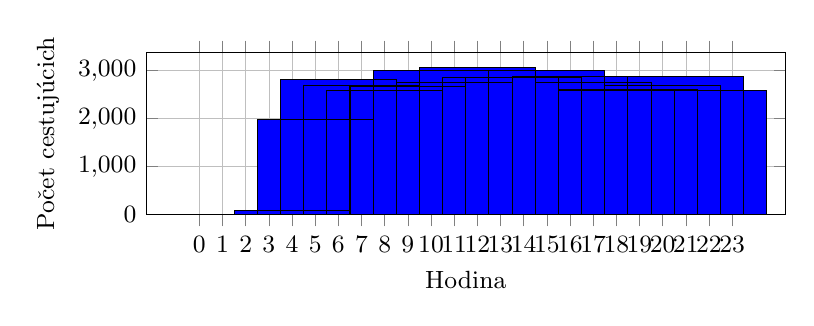
\begin{tikzpicture}
    \begin{axis}[
      width=0.8\textwidth,
      height=0.3\textwidth,
      xlabel={Hodina},
      ylabel={Počet cestujúcich},
      ymin=0,
      xtick={0,1,...,23},
      grid=both,
      major grid style={line width=.2pt,draw=gray!50},
      minor grid style={line width=.1pt,draw=gray!20},
      tick label style={font=\small},
      label style={font=\small},
      legend style={font=\small, at={(0.5,-0.2)}, anchor=north, legend columns=-1},
      ybar,
      bar width=5,
      ]
      \addplot[fill=blue] coordinates {
        (0, 0) (1, 0) (2, 0) (3, 0) (4, 87) (5, 1988) (6, 2803) (7, 2690) 
        (8, 2585) (9, 2673) (10, 3006) (11, 2755) (12, 3067) (13, 2859) 
        (14, 2860) (15, 3005) (16, 2866) (17, 2759) (18, 2593) (19, 2596) 
        (20, 2694) (21, 2874) (22, 2584) (23, 0)
      };
    \end{axis}
  \end{tikzpicture}
  \caption{Počet cestujúcich prichádzajúcich na zastávku za hodinu}
\end{figure}

\begin{figure}[h]
  \centering
  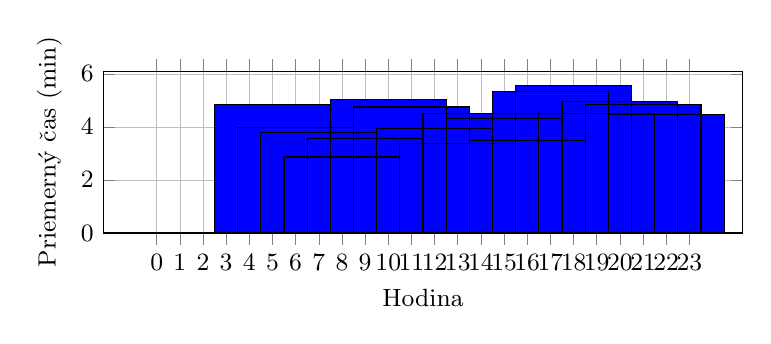
\begin{tikzpicture}
    \begin{axis}[
      width=0.8\textwidth,
      height=0.3\textwidth,
      xlabel={Hodina},
      ylabel={Priemerný čas (min)},
      ymin=0,
      xtick={0,1,...,23},
      grid=both,
      major grid style={line width=.2pt,draw=gray!50},
      minor grid style={line width=.1pt,draw=gray!20},
      tick label style={font=\small},
      label style={font=\small},
      legend style={font=\small, at={(0.5,-0.2)}, anchor=north, legend columns=-1},
      ybar,
      bar width=5,
      ]
      \addplot[fill=blue] coordinates {
        (0, 0) (1, 0) (2, 0) (3, 0) (4, 0) (5, 4.835010060362173) (6, 3.9739564752051373) (7, 3.7762081784386616) 
        (8, 2.8638297872340424) (9, 3.551440329218107) (10, 5.027611443779109) (11, 4.749546279491833) 
        (12, 3.9507662210629277) (13, 3.3823015040223856) (14, 4.488811188811189) (15, 4.311480865224626) 
        (16, 3.4874389392882064) (17, 5.325480246466111) (18, 5.548785190898573) (19, 4.500385208012327) 
        (20, 4.944691907943579) (21, 4.835421016005567) (22, 4.468266253869969) (23, 0)
      };
    \end{axis}
  \end{tikzpicture}
  \caption{Priemerný čas strávený čakaním za hodinu}
\end{figure}


\begin{table}[h]
  \centering
  \begin{minipage}{0.35\textwidth}
    \centering
    \begin{tabular}{|l|c|}
      \hline
      \textbf{Zastávka} & \# \\ \hline
      Židenice, Stará osada & 0 \\ \hline
      Gajdošova & 2 \\ \hline
      Otakara Ševčíka & 3 \\ \hline
      Škroupova & 4 \\ \hline
      Tržní & 6 \\ \hline
      Hladíkova & 8 \\ \hline
      Autobusové nádraží & 10 \\ \hline
      Opuštěná & 12 \\ \hline
      Křídlovická & 15 \\ \hline
      Poříčí & 16 \\ \hline
      Mendlovo náměstí & 20 \\ \hline
      Křížkovského & 21 \\ \hline
      Výstaviště & 22 \\ \hline
      Riviéra & 24 \\ \hline
      Pisárky & 26 \\ \hline
      Anthropos & 28 \\ \hline
      Pod Jurankou & 29 \\ \hline
      Veslařská & 30 \\ \hline
      Jundrov, hřiště & 31 \\ \hline
      Jundrovský most & 32 \\ \hline
      Vozovna Komín & 34 \\ \hline
      Hlavní & 35 \\ \hline
      Štursova & 36 \\ \hline
      Rosického náměstí & 37 \\ \hline
      Přívrat & 39 \\ \hline
      Záhřebská & 40 \\ \hline
      Skácelova & 42 \\ \hline
      Slovanské náměstí & 43 \\ \hline
      Husitská & 44 \\ \hline
      Semilasso & 46 \\ \hline
      Královo Pole, nádraží & 47 \\ \hline
      Mojmírovo náměstí & 48 \\ \hline
      Kociánka & 49 \\ \hline
      Královopolská strojírna & 50 \\ \hline
      Divišova čtvrť & 51 \\ \hline
      U Tunýlku & 52 \\ \hline
      Halasovo náměstí & 54 \\ \hline
      Poliklinika Lesná & 55 \\ \hline
      Lesná, nádraží & 56 \\ \hline
      Štefánikova čtvrť & 57 \\ \hline
      Merhautova & 59 \\ \hline
      Tomkovo náměstí & 61 \\ \hline
      Židenice, kasárna & 63 \\ \hline
      Židenice, Stará osada & 65 \\ \hline
    \end{tabular}
    \caption{Rozpis zastávok}      
  \end{minipage}
  \begin{minipage}{0.55\textwidth}
    \centering
    \begin{tabular}{|c|l|}
      \hline
      \textbf{h} & \textbf{Odchody} \\ \hline
      05 & 00, 07, 15, 22, 30, 37, 45, 52 \\ \hline
      06 & 00, 08, 17, 25, 34, 42, 51 \\ \hline
      07 & 00, 05, 10, 16, 21, 27, 32, 38, 43, 49, 54 \\ \hline
      08 & 00, 06, 12, 18, 24, 30, 36, 42, 48, 54 \\ \hline
      09 & 00, 10, 20, 30, 40, 50 \\ \hline
      10 & 00, 10, 20, 30, 40, 50 \\ \hline
      11 & 00, 08, 17, 25, 34, 42, 51 \\ \hline
      12 & 00, 06, 12, 18, 24, 30, 36, 42, 48, 54 \\ \hline
      13 & 00, 08, 17, 25, 34, 42, 51 \\ \hline
      14 & 00, 10, 20, 30, 40, 50 \\ \hline
      15 & 00, 05, 10, 16, 21, 27, 32, 38, 43, 49, 54 \\ \hline
      16 & 00, 10, 20, 30, 40, 50 \\ \hline
      17 & 00, 12, 24, 36, 48 \\ \hline
      18 & 00, 08, 17, 25, 34, 42, 51 \\ \hline
      19 & 00, 10, 20, 30, 40, 50 \\ \hline
      20 & 00, 10, 20, 30, 40, 50 \\ \hline
      21 & 00, 08, 17, 25, 34, 42, 51 \\ \hline
      22 & 00, 07, 15, 22, 30, 37, 45, 52 \\ \hline
    \end{tabular}
    \caption{Časový rozpis}
  \end{minipage}
\end{table}
